\documentclass{ximera}
%herschreven 23 september 2026
\title{Homogeen veld}
\author{Daan Lipkens}

\begin{document}
\begin{abstract}
    
\end{abstract}
\maketitle
%———————————————————————————————————————

\begin{proposition}[foldable=true]
Een homogeen veld is een veld waarbij de veldvector overal identiek is. Dit betekent:
\begin{enumerate}
    \item zelfde grootte;
    \item zelfde richting;
    \item zelfde zin.
\end{enumerate}
\end{proposition}
Om veldlijnen te tekenen met een zelfde richting en zin, moeten ze evenwijdig zijn met elkaar en alle pijlpunten naar de zelfde kant wijzen. Om de grootte van het veld overal even groot te krijgen, moeten alle veldlijnen even ver van elkaar staan, zoals te zien op figuur \ref{fig:homogeen_elektrisch_veld}.
\begin{remark}[expandable=true]
Een homogeen elektrisch veld wordt gemaakt door twee parallelle platen met een verschillende lading, zoals te zien op figuur \ref{fig:homogeen_elektrisch_veld}, maar ook in de lengte van een stroomvoerende geleider.
\end{remark}
%---------------------------
% AFBEELDING: Homogeen elektrisch veld tussen twee platen (pijlen in het midden)
\begin{figure}[ht!]
    \captionsetup{width=0.85\textwidth}
    \begin{center}
        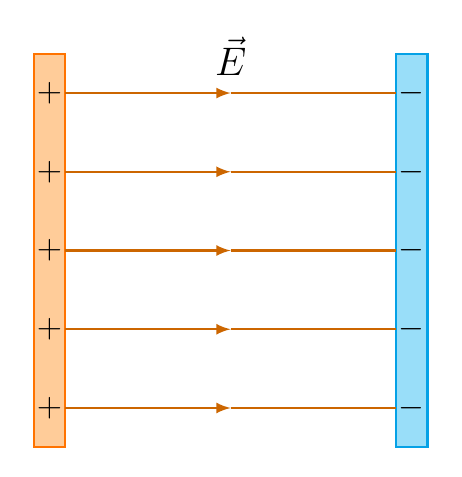
\begin{tikzpicture}[scale=1]

            % Stijlen voor de platen en veldlijnen
            \tikzset{
                posplate/.style={fill=orange!40, draw=orange!90!red, thick},
                negplate/.style={fill=cyan!40, draw=cyan!90!blue, thick},
                fieldline/.style={thick, orange!80!black}
            }

            % --- PLATEN TEKENEN ---
            % Linkerplaat (Positief)
            \draw[posplate] (-2.5, -2.5) rectangle (-2.1, 2.5);

            % Rechter plaat (Negatief)
            \draw[negplate] (2.1, -2.5) rectangle (2.5, 2.5);

            % --- LADINGEN (PLUS EN MIN) TOEVOEGEN ---
            \foreach \y in {-2, -1, 0, 1, 2} {
                \node[font=\large] at (-2.3, \y) {$+$};
                \node[font=\large] at (2.3, \y) {$-$};
            }

            % --- VELDLIJNEN TEKENEN ---
            % Evenwijdige lijnen op gelijke afstand van elkaar
            \foreach \y in {-2, -1, 0, 1, 2} {
                % Deel 1: Van linkerplaat tot halverwege met een pijl
                \draw[fieldline, ->, >=latex] (-2.1, \y) -- (0, \y);
                % Deel 2: Vanaf halverwege tot aan de rechter plaat
                \draw[fieldline] (0, \y) -- (2.1, \y);
            }

            % --- LABEL VOOR HET ELEKTRISCH VELD ---
            % We zetten de E-vector netjes bovenaan, iets boven de bovenste veldlijn
            \node[above, font=\Large] at (0, 2.1) {$\vec{E}$};

        \end{tikzpicture}
    \end{center}
    \caption{Een homogeen elektrisch veld $\vec{E}$ tussen twee evenwijdige geladen platen. De veldlijnen lopen evenwijdig en op gelijke afstand van elkaar, wat aangeeft dat het veld overal even sterk is.}
    \label{fig:homogeen_elektrisch_veld}
\end{figure}
%---------------------------
\end{document}